\graphicspath{ {img/MAB_CSSA/} }
\chapter[A superprocess with Upper Confidence Bounds for Cooperative Spectrum Sharing][A superprocess with UCB for CSS]{A superprocess with Upper Confidence Bounds for Cooperative Spectrum Sharing}\label{MAB_CSSA_chap}

\section{Introduction}

The demand for wireless communications has kept growing in the recent years, to the point of making the traditional fixed licensing process obsolete \cite{ref:Valletti2001,ref:Jorswieck2013}. 
In an effort to devise more efficient management of spectrum access, dynamic spectrum access (DSA) policies have been proposed \cite{ref:Zhao2007_sur}. 
DSA allows secondary users (SUs) without license to opportunistically access the spectrum, sparsely used by the primary users (PUs). 
A subset of these policies, spectrum trading policies \cite{ref:Mario2014}, aim to create a highly dynamic market of spectrum.
Among other proposed solutions, spectrum trading has a key advantage: it provides the primary users with economic and/or any other incentives to allow access to their resources. 

Our work is in the framework of \textit{Cooperative Spectrum Sharing} (CSS), also known as \textit{Cooperative Secondary Spectrum Access} () or \textit{Cooperative Cognitive Radio Networks} (CCRNs). 
More specifically, we are interested in the trading scenario introduced by \cite{ref:Simeone2008}. 
The basic premise of CSS is that secondary users (SUs) without license may act as transmission relays for a licensed primary transmitter (PT) in exchange of transmission opportunities in the spectral resources of the PT.

CSS is different from other market-driven spectrum sharing approaches in that it fosters the creation of transmission opportunities in the PU spectrum in an exogenous way: by increasing the transmission rate of the PU, it reduces its spectrum usage. 
Because of that, CSS is particularly useful when the PU own demands are so high that it would rarely have spectrum to lease.
\footnote{It could be the case that the PU has a low traffic volume and it is not interested in increasing its transmission rate. 
For that reason, hybrid approaches combining CSS and other DSA ideas, with monetary transactions, have also being studied \cite{ref:Zhang2009,ref:Zhang2012_Fair}.}

\subsection{Motivation}
A CSS system poses the following \textit{key challenges}: 1) spectrum resource allocation; 2) the SUs may belong to self-interested networks different from the PT's, and thus, the PT should not expect the SUs to collaborate in maximizing the PT's profit; 3) the PT has to undergo a negotiating process with the nearby SUs, having no previous information about them, in general; 4) spectrum opportunities may happen on a short timescale (of the order of seconds or less), thus, for CSS to be effective, this negotiation must be carried out in real-time; 5) the situation around the PT can change quickly (\textit{e.g.,} SUs arriving and leaving the system). 

Previous works in CSS have not addressed these issues simultaneously. As we discussed in \cite{ref:Mario2014} and we explain in Section \ref{sec:Rel}, they are focused on requirements 1-3, but the time needed to reach elaborated solutions (requirements 4 and 5) is not considered enough. 
Multiple factors in spectrum trading (\textit{e.g.,} supply, demand, channel gains) vary rapidly with time, and trying to reach a complex allocation solution for a particular spectrum opportunity could take so long that it may render the solution impractical.

We focus on meeting all the aforementioned requirements from the perspective of a PT, requesting help from SUs to communicate with an intended primary receiver (PR). The PT has to gradually learn the optimal SU - offer combination based on its accumulated observations. Our proposal aims to achieve a balance between the time devoted by the PT to exploration of options and the time spent exploiting the best alternative known so far, to maximize the PT's payoff (in terms of net transmitted data) over time.

\subsection{Contribution}

\textit{We develop a new approach for the PT learning problem in the context of CSS}, by means of a stochastic multi-armed bandit problem (MAB) with dependent arms. This approach allows the PT to group the information gathered from SUs instead of treating every possible action independently. Thus, the PT learns in a more efficient way from its observations with respect to other reinforcement learning approaches. We formulate the main problem in Section \ref{sec:Sys}.
The reward function of our MAB comprises two factors: one is drawn from a probability distribution, and the other one is determined by a Markov chain.
To the best of our knowledge, there are no algorithms in previous literature for this type of rewards in MABs. 
In Section \ref{sec:MAB}, \textit{we describe our MAB-MDP algorithm} (to be presented in \cite{ref:Mario2015}), in which we integrate a stochastic MAB and an MDP. MAB-MDP allows us to introduce some key concepts used in Section \ref{sec:Super}, to build \textit{a new algorithm, Super-UCB, for solving the stochastic MAB with dependent arms.} This algorithm combines traditional indices used in stochastic MABs \cite{ref:Auer2002}, known as Upper Confidence Bounds, and an extension to markovian MABs \cite{ref:Gittins2011} called superprocess. \textit{Super-UCB makes a more efficient use of the available information, achieving a better performance without increasing the computational overhead.} \textit{We evaluate the performance, scalability and robustness of Super-UCB with Monte Carlo simulations} in Section \ref{sec:Num}.
Our solution is not only directly implementable, without strong assumptions, but also extensible to more complex scenarios, as summarized in the conclusions in Section \ref{sec:Con}.

% All agents are considered to be self-interested, in that they look for their own profit only. 
% In each transmission period, the PT has to choose an SU to act as a relay, and make this SU an offer in terms of SU transmission time.
% The PT obtains a payoff in terms of net transmitted data.
% The average path loss of each SU-PR channel are initially unknown by the PT. 
% The PT also ignores the offers that each SU would be willing to accept. 
% Therefore it has to gradually learn the optimal SU - offer combination based on the accumulated observations. 
% Because in a realistic setting the situation around the PT can change quickly (\textit{e.g.,} SUs arriving and leaving the system), our proposals aim to achieve a balance between the time devoted by the PT to exploration of options and the time spent exploiting the best alternative known so far, to maximize the PT's payoff over time.

\section{Related Work}\label{sec:Rel}
\begin{table*}
\begin{threeparttable}
\caption{Summary of related works}
\label{MAB_CSSA_table_related_work}
\begin{tabular}{|p{1.7cm}|*{7}{p{1.75cm}|}}
\hline
    & Our work & \cite{ref:Feng2014} & \cite{ref:Duan2014} & \cite{ref:Yan2013} & \cite{ref:Zhang2012_Fair} & \cite{ref:Yi2010} &  \cite{ref:Yuan2013} \\\hline

Information & \textbf{Strongly incomplete} & Incomplete & Incomplete & Incomplete & Complete & Complete & Complete \\\hline
Learning & \textbf{Exploration - exploitation} & Greedy search & No & \textbf{Repeated game} & N/A & N/A & N/A \\\hline
Penalization for rejected offers & \textbf{Yes} & No & N/A & \textbf{Yes} & N/A & N/A & N/A \\\hline
Communication & \textbf{Unicast} & Broadcast & Broadcast & \textbf{Unicast} & Broadcast & Broadcast & Broadcast \\\hline
Technique & \textbf{MAB - superprocess} & Matching Th. & Contract Th. & Bargaining & Co-op. bargaining & Stackelberg game  & MILP optimization\\\hline
Market form & \textbf{1 PU - n SUs} & \textbf{1 PN - n SUs} & \textbf{1 PU - n SUs} & 1 PU - 1 SU & \textbf{1 PU - n SUs} & 1 PN - 1 SN & n PUs - n SUs\\\hline
Objective & \textbf{Max. PU reward} & \textbf{Max. PU reward} & \textbf{Max. PU reward} & Equilibrium (bias towards SUs) & Max. SU rewards and fairness & Equilibrium (bias towards PU) & Configurable \\\hline
Year & \textbf{2014} & \textbf{2014} & \textbf{2014} & 2013 & 2012 & 2010 & 2013\\\hline
\end{tabular}
\begin{tablenotes}
\item \hspace{5em} N/A = Not applicable, PN = Primary Network, SN = Secondary Network, MILP = Mixed Integer Linear Programming
\end{tablenotes}
\end{threeparttable}
\end{table*}
Many previous works in CSS such as \cite{ref:Simeone2008,ref:Zhang2009,ref:Yi2010,ref:Nadkar2011} consider perfect information scenarios. 
They assume global knowledge of the network, actions and payoffs of other entities present in the system, and even private information like the value an entity gives to the traded good.
It is unlikely that the SUs belonging to a different operator would reveal private information to the PT, taking into account that they may obtain higher payoffs by hiding it or even lying, at the cost of worsening the whole system. 
Some of this private information, in addition, is non-mensurable. For example, if a PT suspects an SU is lying about its transmission power, it could check what the transmission power of an SU is, but there is no way to know how much battery it has left. 
Our incomplete information scenario is stronger than most works addressing this issue. 
For example, we do not assume any value range for received powers unlike \cite{ref:Feng2014}, and completely rely on learning to discover them. 

Other approaches like the ones proposed in \cite{ref:Yuan2013,ref:Han2010,ref:Li2011} consider cooperation between networks belonging to different operators. 
Although it is possible to design mechanisms that provide incentives to selfish SUs to collaborate with the PT (cooperation in terms of game theory \cite{ref:Zhang2012_Fair}), they require the exchange of several messages between these individuals, and therefore a loss in transmission efficiency, as pointed out in \cite{ref:Niyato2008}.

These selfish entities, however, do have incentives to make strategies and/or collude against the PT. 
In our proposal the PT employs one-to-one bargaining instead of broadcast offers, as \cite{ref:Yan2013}, but we consider more than one SU. The benefits of one-to-one transactions versus broadcast mechanisms \cite{ref:Feng2014,ref:Duan2014,ref:Jayaweera2011,ref:Zhang2009,ref:Simeone2008} are: the reduction of the strategic power of the SUs, as they cannot overhear public offers or other information about their competitors; their robustness against collusions of SUs \cite{ref:Alcaraz2014_coa}; and the reduction of the communication overhead on the control channels in comparison to widespread mechanisms such as auctions \cite{ref:Feng2014, ref:Jayaweera2011} (\textit{e.g.,} multiple rounds of bidding messages).
 
Auction mechanisms are also a popular approach to handle the incomplete information issues in CSS.
Truthful auctions allow optimal solutions without assuming the knowledge of private information, but at the cost of complex winner-selection algorithms and/or increased communication overheads. 
This may not be suitable for spectrum trading in short timescales. There are other mechanisms such as \cite{ref:Duan2014}, in which the authors do not assume perfect information and are concerned about the complexity of the algorithm. They develop a stochastic optimization based on contract theory. Nevertheless, in contrast to our proposal, they do not implement any learning process from successive interactions with SUs. Independent learning is a key feature of self-organizing networks and scalability, as indicated in the survey on market mechanisms assuming incomplete information for CSS in \cite{ref:Huang2013}.

Our work is inspired by \cite{ref:Yan2013}, where the authors consider CSS between a PU and a cognitive SU pair in a repeated bargaining game. 
The bargaining partner selection problem in our work is not comparable to the one formulated in \cite{ref:Calvo2002} because we do not assume knowledge about the impatience of other players, and we consider the PU has full bargaining power and learning abilities, among other differences. 
Bargaining partner selection is also different from traditional best-relay selection problems in multi-hop networks or cooperative networks \cite{ref:Yuan2013,ref:Tran2014}, which expect a internetwork collaborative behavior in the form of relays revealing their true link qualities, battery life, etc.

Our research in this paper is built on the techniques for multi-armed bandit with dependent arms developed by D.B. Brown and J.E. Smith in \cite{ref:Brown2013} and S. Pandey, D. Chakrabarti and D. Agarwal in \cite{ref:Pandey2007}. In \cite{ref:Brown2013}, a MAB superprocess is used to develop an optimal policy for exploring oil and gas fields in the North Sea. The state space of their problem is finite, unlike ours. 
Our dependency model is also different enough from \cite{ref:Pandey2007} to require substantial changes in their algorithm, such as the integration with an MDP. 
Multi-armed bandits have been previously used in spectrum sharing, mainly for sensing or resource allocation \cite{ref:Si2010}. 
Surveys on bandits and other machine learning algorithms in cognitive radio can be found in \cite{ref:Bkassiny2013} and \cite{ref:Gavrilovska2013}.
To the best of our knowledge, however, this it the first work exploiting MABs in CSS. 

Other related works explore alternative flavors of CSS. For example \cite{ref:Tran2014} explores the possibility of both PUs and SUs acting as relays of each other assuming a cooperative attitude between them. 
The work in \cite{ref:Shao2014} shows the optimal strategy of a SU which is allowed to dynamically decide whether it enters a CSSs or a spectrum leasing market. A close related topic to CSS is the overlay cognitive radio network paradigm \cite{ref:Goldsmith2009}, by which a SU acts as relay for the PU and, at the same time, transmits its own message. 
The interference constraint on the SU transmission is enlarged thanks to the cooperative transmission and the use of interference cancellation techniques \cite{ref:Han2010}. 

Table \ref{MAB_CSSA_table_related_work} summarizes the most significant features of our paper and compares it to previous works. 
Note that for those works analyzing different configurations, we select and compare to the one closest to our proposal. 

\section{System Model}\label{sec:Sys}

\begin{figure}[!t]
\centering
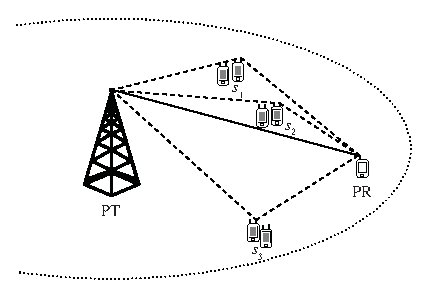
\includegraphics{geo.eps}
\caption{Cooperative Spectrum Sharing.}
\label{fig:geo}
\end{figure}

The protocol considers a PU transmitter (PT) - receiver (PR) pair and a set of SU cognitive pairs in the coverage area of the PT denoted by $\mathcal{S}\equiv\left\{s_1,s_2,\ldots,s_S\right\}$, as in Fig. \ref{fig:geo}.
The system is under the ``exclusive-use'' coexistence model by which the PUs are the only entities with the right to transmit in a certain band. 
When the PU pair's channel conditions are not suitable for direct transmission, the PT would be willing to use the SUs as relays.

In exchange for its services, the PT makes an offer to the SU, consisting of a certain amount of time for SU data transmission over the PU channels. 
The SUs transmit with fixed power, the same for relaying and their own transmissions. 
%The SUs are interested in extra transmission opportunities but they are assumed to have their own resources.
The SUs are assumed to have their own, but limited, spectral resources. Therefore, although it is not crucial for their communication purposes, the SUs may benefit from the additional spectrum resources obtained from the PU.
As a consequence, it is the PT who contacts the SU and initiates the bargaining.

Time is divided into fixed transmission periods or \textit{frames}, which we will consider of duration $T = 1$ units of time and numbered as $n=1,2,\ldots$. 
The offer that the PT makes, denoted by $\alpha \in [0,1]$, is the fraction of the transmission period during which the SU is allowed to transmit its own data.
For tractability, we discretize that interval in equal increments and $\mathcal{A}_s = \left\{\alpha_{1},\ldots,\alpha_{A}\right\}$ denotes the set of possible offers to make to SU $s \in \mathcal{S}$.\footnote{In practice we will assume $\alpha_A = 0.9$, and $\alpha_1>0$, as neither the SU nor the PT may ``work for free''.} 

Each transmission period is composed of a decision phase, an optional bargaining phase, and a communication phase as in \cite{ref:Simeone2008,ref:Yan2013}, see also Fig. \ref{fig:phase}. 

\begin{figure}[!t]
\centering
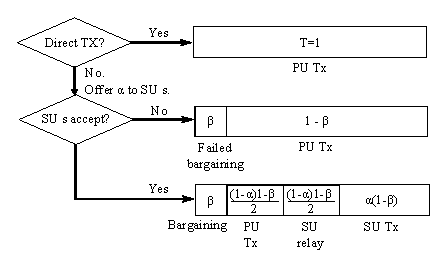
\includegraphics{phase.eps}
\caption{Frame structures.}
\label{fig:phase}
\end{figure}

\begin{itemize}
\item Decision phase. During this phase, the PT has to choose which SU to bargain with and what offer to make to it: $(s,\alpha)\in\underset{s\in\mathcal{S}}\bigcup s\times\mathcal{A}_s$. The PT aims to maximize its accumulated payoff, and its decisions are based on previous interactions.
\item Bargaining phase. We consider the PT has full bargaining power and makes a take-it-or-leave-it offer to a SU. This phase models the time spent in sending that message and waiting for the answer. 
\item Communication phases. If the offer is rejected by the SU, the PT directly transmits for the rest of the frame to its intended receiver. 
If the offer is accepted by the SU, then the comunication phase is divided into three time periods: 
\begin{itemize}
\item Direct transmission of the PT. The PT transmits its information to its receiver and to the selected SU.
\item SU forwarding. The selected SU re-transmits the information to the PR.
\item SU own transmission.
\end{itemize}
\end{itemize}

\subsection {Payoff Functions}

\textbf{PT's Payoff.} For the cooperative transmission, the system employs the decode and forward relay communication scheme from \cite{ref:Laneman2001}. 
For a given $s\in\mathcal{S}$, the links initially involved are: PT-PR, PT-$s$, and $s$-PR. Let $\Gamma_{\text{P,P}}$, $\Gamma_{\text{P,}s}$, and $\Gamma_{s}$ be their respective average SNR values.
The achievable data rate satisfies
$R_{\text{P}}^{s} = C\min\{\log(1+\Gamma_{\text{P,}s}),\log(1+\Gamma_{\text{P,P}}+\Gamma_{s})\}$, where $C$ is a constant.
We assume that the SUs always decode the PT data correctly in the first phase, and thus we focus on the $s$-PR link and 
%This assumption is justified by the fact that, as noticed in \cite{ref:Duan2014}, the SUs involved in relaying the signal will probably be the ones closer to the PU transmitter\footnote{Because they are the ones which can ``hear'' the request of the PT.}, and the SU-PR channel becomes the bottleneck
%\footnote{It is worth noting that the period of time of direct transmission and the period of SU acting as relays should not be necessarily equal, as this would depend on the achievable data rates of those links and could be optimized, or even learned in an online manner.}. 
we have 
$R_{\text{P}}^{s} = C\log(1+\Gamma_{\text{P,P}}+\Gamma_{s})$.
Since the PT-PR and s-PR links are considered to be in bad and good propagation conditions respectively, \textit{i.e.,} $\Gamma_{\text{P,P}}\ll\Gamma_{s}$, and $1 \ll\Gamma_{s}$, the achievable data rate can be approximated as
$R_{\text{P}}^{s} \approx C\log(\Gamma_{s})$.

The time allocated to the $s$-PR transmission within a frame can be considered long compared to fast fading variations. That is, the effect of multipath is assumed to be negligible in terms of the average SNR, $\Gamma_s$. Therefore, $\Gamma_s$ is mainly determined by pathloss attenuation and shadowing, remaining constant during an s-PR transmission. Successive SU relay phases between $s$ and the PR are sufficiently distant in time for the channel to decorrelate. Thus, the SNR samples $\Gamma_s^{(n)}$ are modeled as i.i.d. random variables, following a log-normal distribution which typically characterizes shadowing \cite{ref:Goldsmith2009}, \textit{i.e.,} $\log(\Gamma_s^{(n)})=\gamma_s^{(n)} \sim N(\mu_{\gamma_s},\sigma_{\gamma_s})$. 

%\footnote{Another interesting approach could be imposing a target data rate transmission to the SU relay, without CSI, and not assuming that $\gamma_{s}$ can be observed, but just if a packet arrived correctly or incorrectly (outage). The problem would be learning the outage probabilities of each SU for that target rate, and possibly studied with a Bernoulli-MAB. In such scenario, the variances of the SNRs would have a greater impact.}%
The PR can observe the value of $\gamma_s^{(n)}$ and feed it back to the PT at the end of each transmission frame. Then, the reward for the PT in frame $n$ is the transmission rate it gets, multiplied by the time that transmission lasts:
\begin{equation}\label{eq:W}
W^{(n)}(s,\alpha) = \left\{ 
  \begin{array}{l l}
    (1-\beta)(1-\alpha)\log({\Gamma_s^{(n)}}) & \text{  } \text{if } \alpha \text{ is accepted}\\
    (1-\beta)\log(1+\Gamma_{P,P}^{(n)}) & \text{  } \text{otherwise}
  \end{array} \right.
\end{equation}
For the sake of clarity, from now on we set $\beta=0$ and $\log{(1+\Gamma_{P,P}^{(n)})} = 0$ for all $n$. Nevertheless, our model is also applicable with different values of these parameters. 

%We can define the utility function of the PT as $U_p(u^{(1)},\ldots,u^{(n)}) = \mathbb{E}\left[\sum_{k=1}^{n} W(u^k)\right]$, for an unknown, finite time horizon $n$.

%An SU, $s$, can be aware of actual channel gain at the $s$-PR link (for example, using a pilot signal) but does not disclose this information to the PT. %The outage probability of its transmission is negligible. If the channel is in deep fading during a frame, the achieved data rate will be low.
%In Section \ref{sec:Det}, that measure is the true average received SNR (for example, an accurate estimation of the SU). In Section \ref{sec:Sto}, that measure will be a sample drawn from the log-normal distribution characterizing the received SNR from that SU.

\textbf{SU's Payoff.} The payoff obtained by an SU acting as relay is the difference between the its net transmitted data during a frame when using the PT channel, $\alpha R_{s}^{\text{P}}$, and the net data it would transmit when using its own spectral resources $R_{s,s}$. An SU accepts any offer providing positive payoff, resulting in a threshold behavior. SU $s$ accepts an offer $\alpha_a$ whenever $\alpha\geq \alpha_s^{th}$, where $\alpha_s^{th}$ is the offer that gives the SU zero payoff. We define the \textit{type of an SU} as the index $a$ of the smallest $\alpha_{a}\in\mathcal{A}_s$ that this SU will accept. 
%As an example, if we consider 4 possible offers, then $\mathcal{A}_s = \{0.3,0.5,0.7,0.9\}$.
%An SU of type 1 will accept all offers, type 2 will accept from 0.5 onwards (0.7 and 0.9), and type 4 will only accept the greatest offer 0.9. All SUs accept at least the greatest offer 0.9.
%%We can justify this fixed threshold behavior with the following reasoning. Let us assume that using their own spectrum resource, SUs achieve data rate $R_{s}^{own}$ and the data rate they achieve using the PU resources is $R_{s}^{PU}$.
%%Then, we could see that an SU will accept a PU offer if the following condition holds:
%%\begin{equation}
%%\alpha \geq \frac{R_{s}^{PU}}{(1-\beta)R_{ss}} = \alpha_{s}^{\text{th}}
%%\end{equation}
If the link between the SU pair is stable (\textit{e.g.,} a close ad hoc connection) and the offered PU bandwidth is constant (only the time offered changes), the thresholds, and therefore the type of each SU, remain constant over multiple transmission frames.
% \subsection {Primary User Model}
% For the cooperative transmission, the system employs the decode and forward relay communication scheme from \cite{ref:Laneman2001}. The achievable data rate satisfies:
% \begin{equation} 
% R_{PT} = \frac{1}{2} \min\{\log(1+\gamma_{PT,ST}),\log(1+\gamma_{PT,PR}+\gamma_{SU,PR})\}
% \end{equation}
% where $\gamma_{A,B}$ is the SNR measured at terminal $B$ from terminal $A$.
% We consider the SUs always decode the PT's data correctly in the first phase, and thus, we focus on the relay link between an SU and the PR. 
% This assumption is justified by the fact that, as noticed in \cite{ref:Duan2014}, the SUs involved in relying the signal will probably be the ones closer to the PU transmitter \footnote{Because they are the ones which can ``hear'' the request of the PT}, and the SU-PR channel becomes the bottleneck\footnote{It is worth noting that the period of time of direct transmission and the period of SU acting as relays should not be necessarily equal, it would depend on the achievable data rates of those links and could be optimized, or even learned in an online manner}. Thus, we will consider: 
% \begin{equation}
% R_{PT} = \log(1+\gamma_{PT,PR}+\gamma_{SU,PR})
% \end{equation}
% And as we stated before, we will assume the direct channel transmission is always in bad condition. The achievable data rate would then be that of the channel between the relay and the PR:
% \begin{equation}
% R_{PT} = \frac{1}{2} \log(1+\gamma_{SU,PR}).
% \end{equation}


% The SU - PR links are modeled as block shadow fading channels. 
% During a transmission frame, we assume $\gamma_{SU,PR}$ remains constant and changes randomly at the next frame following a log-normal distribution.
% That distribution has different mean values for the different SUs and, without loss of generality, we will consider they all experience the same variance. 
% We assume the SUs have full CSI (Channel Side Information) so that they could transmit adapting the data rate to the current channel gain with negligible outage probability.  
% We consider the PU has no special requirements on the delay or the need of a constant data rate (as in voice applications).
% We also consider the PR can observe the value of the SNR after packet reception and feed it back to the PT\footnote{Another interesting approach could be imposing a target data rate transmission to the SU relay, without CSI, and not assuming the SNR can be observed, but just if a packet arrived correctly or incorrectly (outage). The problem would be learning the outage probabilities of each SU for that target rate, and possibly studied with a Bernoulli-MAB). In such scenario, the variances of the SNRs would have a greater impact}. Then, it makes sense to define the utility function as:
% \begin{equation}
% U_{PU} = (1-\alpha)\log(\gamma_{ST,PR}).
% \end{equation}

% \subsection {Secondary User Model}
% In this section we will describe the SU model we assume.
% The SUs transmit with fixed power but each SU in the PT coverage area have different channel gains to the PR. Because of that, the reward received by the PT when using each of them as relays will be different, and not only in the offers they accept.

% The SU has knowledge of the actual value of its channel gain (for example, using a pilot signal) but does not disclose that information to the PT. The outage probability of its transmission is negligible. If the channel is in deep fading during a frame, simply the achieved data rate will be low.

% Upon arrival to the system, the SUs communicate with the PU pair, so that the PR gets a measure of the average receive SNR it can expect from that particular SU. \footnote{We could also leverage this constraint by simply assuming an initial belief (with much uncertainty) about a SU. However, this initial sample is a common practice in most multi-armed bandit algorithms, whose initialization is by pulling all arms first}. In Section \ref{sec:Det}, that measure is the true average received SNR (for example, an accurate estimation of the SU). In Section \ref{sec:Sto}, that measure will be a sample drawn from the log-normal distribution characterizing the received SNR from that SU. 

% Regarding the SUs' utilities and reaction to the offers of a PT, we assume they exhibit a ``threshold'' behavior: there is a price point below which they will reject all offers.

% As we will discretize the offers the PU can make in the range $\alpha \in [0.1,0.9]$, we define the \textit{type of a SU $\theta$} as the index of the price point, the smallest $\alpha$ offer that it will accept. 
% As an example, if we consider 4 possible offers, then $\mathcal{A}_s = \{0.3,0.5,0.7,0.9\}$.
% An SU of type 1 will accept all offers, type 2 will accept from 0.5 onwards (0.7 and 0.9), and type 4 will only accept the greatest offer 0.9.
% Without loss of generality, we will further consider that all SUs accept at least the greatest offer 0.9.

% We assume the type of a particular SU will remain constant throughout the analysis. We can justify this fixed threshold behavior with the following reasoning. Let us assume that using their own spectrum resource, SUs achieve data rate $R_{s}^{own}$ and the data rate they achieve using the PU resources is $R_{s}^{PU}$.

% We denote the payoff of a SU acting as relay as the difference between the achievable data rate with the help of the PU, and with their own means: 
% \begin{equation}
% U_{SU} = (1- \beta) \alpha R_{s}^{PU} - R_{s}^{own}
% \end{equation}
% Then, we could see that an SU will accept an PU offer if the following condition holds:
% \begin{equation}
% \alpha \geq \frac{R_{s}^{PU}}{(1-\beta)R_{ss}} = \alpha_{s}^{th}
% \end{equation}

% Furthermore, if we assume the link between the SU pair is stable (\textit{e.g.} a close ad-hoc connection) and the offered PU bandwidth is constant (only the time offered changes), we can assume the threshold will be constant.

\subsection {Multi-armed bandit formulation}
Mathematically, we model the sequential decisions of the PT as a multi-armed bandit (MAB) problem.
The PT selects SU-offer pairs $(s,\alpha)$ from the action set $\mathcal{U}=\underset{s\in\mathcal{S}}\bigcup s\times\mathcal{A}_s$.
In the MAB model each $u = (s,\alpha)$ is an arm, and $\mathcal{U}$ is the set of arms.
%For a given $u=(s,\alpha)\in\mathcal{U}$, 
%At each decision round $n$, the PT selects one SU-offer pair $u^{(n)} = (s^{(n)},\alpha^{(n)})\in\mathcal{S}\times\mathcal{A}_s$.
%In the MAB model, each $u = (s,\alpha)$ pair is an arm, and $\mathcal{U}=\mathcal{S}\times\mathcal{A}_s$ is the set of arms.
%Let us denote the set of SUs present in the system as $\mathcal{S}$, and the set of possible offers as $\mathcal{A}_s$. 
%Our MAB problem consists of $|I|$ arms, where the set of arms $\mathcal{U}$ consists of the cartesian product of SUs and possible offers: $\mathcal{U} = \mathcal{S} \times \mathcal{A}_s$.
%Upon the start of each frame $n = 1,2,\ldots$, the PU chooses to pull one of the arms (pick an SU and an offer) and receives a reward $W$, that equals the utility of the PU:
At round $n$, the arm pulled is $u^{(n)} = (s^{(n)},\alpha^{(n)})$, and the reward received by the PT is $W^{(n)} = W^{(n)}(u^{(n)})$.
The history of the system up to time $n$ is defined as the sequence of decisions and observed rewards $W^{(0)},u^{(1)}, W^{(1)},\ldots u^{(n)}, W^{(n)}$ (where $W^{(0)}$ corresponds to initial samples $\gamma_s^{(0)}$).
A \textit{policy} $\pi$ is a function that, at each round $n$, prescribes a decision $u^{(n+1)}$ based on the history of the system. Therefore $\pi$ induces a history $W^{(0)},u_\pi^{(1)},W_\pi^{(1)},u_\pi^{(2)},W_\pi^{(2)},\ldots$. 
The usual performance metric in learning problems is the \textit{regret}. 
At decision stage $n$, we define the regret of a policy $\pi$ by $r^{(n)} = \max_{u}\mathbb{E}\left[\sum_{k=1}^{n}\left(W^{(k)}(u) - W^{(k)}_{\pi}\right)\right]$.
The regret quantifies the performance loss of a policy with respect to a policy that knows the average values
$\mu_{\gamma_s}$ and the type of each SU.
However, in a realistic setting, the PT has no initial information, and faces the challenge of learning both the SU types and the $\mu_{\gamma_s}$ while trying to maximize the reward. 
This is known as the \textit{exploration - exploitation} tradeoff, which implies finding the optimal balance between getting immediate rewards (pulling the arms that seem to be better in expectation) and gathering additional information to make better decisions in future rounds (pulling arms that seem to be worse initially but could potentially be the best).
%It is worth saying that the expectation taken on $W^k_{\pi}$ includes three random processes taking place: 1) the random values of the rewards, 2) the different decisions of a policy given the different observations and 3) randomized policies (such as the $\epsilon$-greedy policy we use as a comparison in Section \ref{sec:Num}).

Learning about the arms of the MAB should not be treated independently.
The reward obtained from an SU $s$ when offered a particular $\alpha$ provides information about the rewards of all the other offers / associated arms. The following example illustrates why. 

\textbf{Example.}
Consider the following set of offers $\mathcal{A}_s = \{0.3,0.5,0.7,0.9\}$, and assume that the PT's initial beliefs about the probability that an SU, $s\in\mathcal{S}$, is of a particular type are equiprobable, \textit{i.e.,} $P(\alpha_a < \alpha_s^{\text{th}}\leq \alpha_{a+1})=0.25$ for $a=1\ldots A-1; P(\alpha_s^{\text{th}} \leq \alpha_1) = 0.25$. %($P(\theta_s = l) = 0.25, l \in \{1..4\}$).
Thus, the beliefs about the probabilities of acceptance of each offer by $s$ are $P(\alpha_s^{\text{th}}\leq \alpha_1) = 0.25$, $P(\alpha_s^{\text{th}}\leq \alpha_2) = 0.5$, and so forth.
With these probabilities we can build the following initial \textit{belief vector}: $[0.25,0.50,0.75,1]$.
%Then, the probability of acceptance of each offer in $\mathcal{A}_s$ by an unknown SU at the decision round $n$ is $p_n = [0.25,0.50,0.75,1]$
If the PT makes the offer $\alpha = 0.5$ to SU $s$ and $s$ accepts it, then the PT will learn that $s$ is neither type 3 nor type 4. Therefore, the belief vector is updated to $[0.5,1,1,1]$.
In addition, the PT observes a sample of $\gamma_s$ and updates its sample mean $\overline\gamma_s^{(1)}$, affecting the belief about the reward of all the arms $\{(s,\alpha_a)\},\text{ } \forall \alpha_a \in \mathcal{A}_s$ of that SU $s$.

\textbf{Reduced MAB.} In the following sections we explain how, inspired by \cite{ref:Pandey2007} and \cite{ref:Brown2013}, respectively, we handle correlation by grouping the observations of an SU, exploiting mutual information. 
We could think of a reduced MAB with $S$ arms, one for each SU, where each arm integrates the information the PT has observed about each SU up to round $n$, that is, the acceptance and rejection of offers, and the SNR samples $\gamma_s^{(n)}$. We must then answer two questions: \textit{how do we represent an SU in the reduced MAB?} Once an SU has been chosen by means of the reduced MAB, \textit{what offer should the PT make to the selected SU?}.

There are two fundamental problems that prevent us from using previous MABs algorithms. The first problem is that the reward of our model does not match those of previous works. We encode the acceptance and rejection of offers as knowledge states. Thus, under a given policy, we can see the changes in the PT's knowledge as a Markov chain. Then, it is clear by (\ref{eq:W}) that the rewards of our reduced MAB come simultaneously from the probability distribution of $\gamma_s^{(n)}$ and from the Markov process of the knowledge states about the offers. Previous algorithms for MABs model the rewards when pulling an arm as drawn from a probability distribution (stochastic MABs), from a Markov chain (markovian MABs), or chosen by an adversary (adversarial MABs). \textit{There are no algorithms in the literature for mixed stochastic and markovian bandits}. Our proposals combine techniques from both types of bandits to solve the reduced MAB. The \textit{MAB-MDP algorithm} relies on a classic algorithm for stochastic MABs, augmented with an MDP, while the \textit{Super-UCB algorithm} is based on an algorithm for markovian MABs augmented with elements from stochastic MABs. The main difference between our two algorithms is that Super-UCB integrates more information about SUs in the PT's policy than MAB-MDP as we will explain further in Section \ref{sec:MAB}.

The second problem when using classic MAB algorithms in our reduced MAB is that those algorithms only dictate one decision in every round (which arm to pull), whereas the PT needs to make one more decision (the offer to the SU).  The MDP of our MAB-MDP algorithm acts as an additional mechanism to the MAB to obtain such policy. In the case of Super-UCB, we make use of an extended model of markovian MABs which handles MABs whose arms are MDPs instead of plain Markov chains, thus providing a policy for arm and action selection. 

% \subsection {Multi-armed bandit formulation}
% Mathematically, we model the sequential decisions and learning of the PT, choosing a SU to act as relay and what offer to make, as a multi-armed bandit (MAB) problem. 
% Let us denote the set of SUs present in the system as $\mathcal{S}$, and the set of possible offers as $\mathcal{A}_s$. 
% Our MAB problem consists of $|I|$ arms, where the set of arms $\mathcal{I}$ consists of the cartesian product of SUs and possible offers: $\mathcal{I} = \mathcal{S} \times \mathcal{A}_s$.

% In each decision phase $n$, the PU chooses to pull one of the arms (pick a SU and an offer) and it receives a reward $W$, that equals the utility of the PU:

% \[ W(s,\alpha) = \left\{ 
%   \begin{array}{l l}
%     (1-\beta)(1-\alpha)\log(1+\gamma_{ST,PR}) & \quad \text{if } \alpha \leq \alpha_{s}^{th}\\
%     (1-\beta)\log(1+\gamma_{PT,PR})& \quad \text{otherwise}
%   \end{array} \right.\]
	
% where $s \in \mathcal{S}$, $\alpha \in \mathcal{A}_s$.
% In our simulations we will consider that the reward when the offer is rejected is zero and recall that $\beta = 0$.

% The objective of the decision - maker (the PT) is to select one arm per round so that the total expected reward is maximized. This obviously means balancing immediate gains (pulling the arms that seem to be better in expectation) with gaining information to do better decisions in the next rounds (pulling arms that seem to be worse initially but could potentially be the best).
% A typical metric in learning problems is the regret, which is the total performance loss of a policy $\pi^n$ against an optimal policy $\pi^*$ pulling the best arm in average in every slot. The basic formulation of regret is: 
% \begin{equation}
% R^n = \mathbb{E}[\sum_n W^n_{\pi^*} - W^n_{\pi^{n}}]
% \end{equation}
% where
% \begin{equation}
% \pi^* = (s^*,\alpha^*) = \text{arg max}_{s,\alpha} \mathbb{E}[W(s,\alpha)]
% \end{equation}

% It is worth saying that the expectation of $W^n_{\pi^n}$ includes three random fenomena taking place: 1) the random values of the rewards, 2) the different decisions of a policy given the different observations and 3) randomized policies (as the $\epsilon$-greedy policy we use as a comparison in Section \ref{sec:Num}).
% For a detailed explanation of regret concepts, see \cite{ref:Bubeck2012}. 

% If we consider the combination $(s,\alpha)$ an arm of the multi-armed bandit problem, it is clear to see that the learning about the arms should not be treated independently.
% The reward obtained from an SU $s$ when offered a particular $\alpha$ will give the PT information about the rewards it can obtain with all the other offers / associated arms. 
% Let us go back to the example of the possibe offers $\mathcal{A}_s = \{0.3,0.5,0.7,0.9\}$. 
% Let us consider that the PT initial beliefs about the probability that an SU is of a particular type are uniformly distributed ($P(\theta_s = l) = 0.25, l \in \{1..4\}$). 
% Then, the probability of acceptance of each offer in $\mathcal{A}_s$ by an unknown SU at the decision round $n$ is $p_n = [0.25,0.50,0.75,1]$
% If the PT tries $\alpha = 0.5$ with an unknown SU and that SU rejects the offer, then the PT will learn that it is not a type-1 or type-2. Therefore, $p_{n+1} = [0,0,0.5,1]$.
% In addition,  the statistics of the rewards of the arms associated to the same SU (the arms representing a SU and each of the possible offers) are the same, multiplied by the constant $(1-\alpha_{1..4})$. 

% Inspired by \cite{ref:Pandey2007,ref:Brown2013}, we handle correlation by grouping the arms of a SU into \textit{clusters}, exploiting the mutual information. 

% In the following sections we describe two different scenarios addressed in our work: a toy scenario with a deterministic bandit setting, in which we consider the PT to have a full characterization of the distribution of the rewards and only has to discover the best offers to make , and the main scenario, a stochastic bandit configuration, in which we consider the PT also has to learn the mean parameter of the reward distributions as it goes. 

% \section{Deterministic bandit setting}\label{sec:Det}
% \textbf{Formulation as a dynamic program}. Let us consider that the PT knows the average SNR it can obtain from each SU in its coverage area but does not know the type of the SUs. 
% However, the PT has an initial estimation of the probability that each SU type is of a particular type. As an example, we are going to consider an uninformative prior belief, that is to say, we assume that the types are equiprobable. 

% We can formulate the search problem of discovering the optimal (SU,$\alpha$), with an exploration - exploitation trade-off, with dynamic programming (DP).  
% The state of the system, $\boldsymbol{x}$, is the information the PT has over the SUs in the system. We denote the information about a SU with $x_i$. 
% Then $\boldsymbol{x} = (x_1,...x_{|\mathcal{S}|})$, with $\mathcal|S|$ the number of SU pairs in the system. 
% For the case of uniform probabiity of the type of a SU, we encode such state with two variables, $(h_{rej},l_{acc})$. $h_{rej}$ is the index of the highest offer the SU has rejected and $l_acc$ is the index of the lowest offer that it accepted \footnote{High from the perspective of the SU, the one that would yield more profit to it}. 
% Please note that $h_{rej} < l_{acc}$. The PT knows that the SU will accept every offer with index $i \leq l_{acc}$ and reject those with index $i < h_{rej}$.
% %TO-DO: rephrase? Give an example?

% The transition probabilities for a given state are the PT's beliefs about the acceptance probabilities of each offer and SU. We consider the knowledge about SUs is not correlated in any way\footnote{But they could be correlated. For example, the PT may know there are SUs in its coverage area with similar behavior (because of some ``identifier'', such as the device type). In that case, the PT might exploit that correlation, updating its knowledge about all SUs with the same profile after interacting with only one of them.}, therefore, the change in state  $\boldsymbol{x}$ is a change in the state of a chosen SU $x_i$. In our example of assuming the type of a SU uniformly distributed, the acceptance probabilities of a particular SU $P(\alpha_s^{th} \leq \alpha_\pi)$ would be:

% \[ P(\alpha_s^{th} \leq \alpha_\pi) = \left\{ 
%   \begin{array}{l l}
%     0 & \text{for } s_\pi \leq h_{rej}\\
%     1 & \text{for } s_\pi > l_{acc}\\
%     \frac{s_\pi-h_{rej}}{l_{acc}-h_{rej}} & \text{for } h_{rej}>s_{\pi} \geq l_{acc} 
%   \end{array} \right.\]

% We can then formulate the Bellman equation as follows:

% \begin{equation}\label{eq:fullDP}
% V(\boldsymbol{x}) = \max_{i \in \mathcal{S}} \max_{\alpha \in \mathcal{A}_s}
%        \mathbb{E}[W(s,\alpha)+\delta \sum_{\boldsymbol{\tilde{x}} \in \mathcal{X}}
%        V(\boldsymbol{\tilde{x}}(\boldsymbol{x},\alpha))P_{\boldsymbol{x} \boldsymbol{\tilde{x}}}]
% \end{equation}

% where $\mathcal{X}$ denotes the set of all possible states and $\boldsymbol{\tilde{x}}$ represents the next stage state.

% The discount factor controls the balance of exploration - exploitation. Depending on the rate of change of the scenario around a particular PT, it may or may not be worth to spend much time learning about a SU. For example, the lifetimes of SUs in the PT's coverage area could be short (exploration is mostly worthless) or longer (exploitation can be delayed). 

% Although we can characterize the problem with DP, even for a small number of SUs and quantization of offers, it will suffer the curse of dimensionality and the model becomes too large for a exact solution. Let us consider only 4 possible offers: the state space of a single SU is 10. If there are 6 SUs in the coverage area, the state space grows to $10^6$.

% Focusing on the case of known average rewards ($W(s,\alpha) = \mu_{s,\alpha})$, the dynamics of the system are ``known'' (the PT does not have to learn the transition function or the rewards), it is less a learning problem and more a computational efficiency problem. 
% In the context of MABs, these problems are known as \textit{bandit optimization problems} \cite{ref:Tekin2013} or \textit{deterministic bandits}.
\section{MAB - MDP algorithm}\label{sec:MAB}
In this proposal, we handle the reduced MAB as an stochastic MAB to obtain a policy for selecting which SU to bargain with, and integrate it with an MDP for the offer selection.

\textbf{Offer selection policy}.
We are interested in finding a policy $\pi_s^{\text{MDP}}$ that, given an SU $s\in\mathcal{S}$, maps the PT's knowledge about the type of $s$, to the next offer $\alpha$ to $s$.
%We can compute a policy for the PT to select the offers it is going to make to an SU by considering an SU $s$ in isolation.
Given $\alpha$, the reward $g$ that the MDP observes is $(1-\alpha)$ if the offer is accepted, and $0$ otherwise.
Therefore, a given policy $\pi_s^{\text{MDP}}$ induces a sequence of rewards $g^{(1)}, g^{(2)},\ldots,g^{(n)}$.
The uncertainty about the time horizon $n$ is captured by a discount factor $\delta<1$, characterizing the expected lifetime of the system, e.g., the probability that the s-PR pair remains active in each frame.
The search problem of discovering the optimal offer to $s$ consists of finding the policy maximizing $\mathbb{E}\left[\sum_{n=1}^{\infty}\delta^{n}g^{(n)}\right]$.
This problem is formulated as an MDP as follows.
%Let us assume a constant $\gamma_s = c$ for that SU (\textit{e.g.} $c = 1$). 

%We formulate the search problem of discovering the optimal $(\alpha_s^*)$ of SU $s$, with an exploration-exploitation tradeoff, by means of the following discounted Markov Decision Process (MDP) and associated Bellman equation:

%\begin{gather}
%\pi_s^{\mathcal{A}_s} = \argmax_{\pi} \sum_n \delta^{(n)} R(x_i,x_j,\pi(x_i)) \\
%¡V(x_i) = \max_{\alpha_a \in \mathcal{A}_s} \sum_{x_j \in \mathcal{X}} P(x_i,x_j,\alpha_a)(R(x_i,x_j,\alpha_a)+\delta V(x_j))
%\end{gather}

The set of \textit{states} of the MDP for SU $s$, denoted by $\mathcal{X}_s$, are all the possible knowledge states about the type of $s$. Assuming uniform probability for the type of an SU, the state of the MDP is completely defined by a two dimensional vector $x$, whose first element, $x(1)$, contains the index of the highest offer rejected by $s$, and $x(2)$ contains the index of the lowest offer that $s$ accepted.
The PT knows that the SU accepts every offer $\alpha_a$ with index $a \geq x(2)$, and rejects those with index $a \leq x(1)$, $\alpha_a \in \mathcal{A}_s$.
The initial state is $(0,A)$, since the PT does not know anything about rejections initially ($x(1)=0$) and $\alpha_A$ is known to be surely accepted ($x(2)=A$).

Each \textit{transition probability} $P_s(x_i,x_j,\alpha_a)$ from a state $x_i$ to a state $x_j$, with $x_i, x_j \in \mathcal{X}_s$, given an offer $\alpha_a$, is determined by the PT's beliefs about the acceptance probability of the offer $\alpha_a$ at current knowledge state, $x_i$. This probability is defined as:
\begin{equation}
 P(\alpha_s^{\text{th}} \leq \alpha_a|x_i) = \left\{ 
  \begin{array}{l l}
    0 & \text{for } 0 < a \leq x_i(1)\\
    \frac{a-x_i(1)}{x_i(2)-x_i(1)} & \text{for } x_i(1) < a < x_i(2) \\
    1 & \text{for } x_i(2) \leq a \leq A 
  \end{array} \right.
\end{equation}
Therefore, the transition probabilities between every pair of states are given by:
\begin{equation}
 P_s(x_i,x_j,\alpha_a) = \left\{ 
  \begin{array}{l l}
    P(\alpha_s^{\text{th}}\leq\alpha_a|x_i) & \text{for } a = x_j(2)\\
    1 - P(\alpha_s^{\text{th}}\leq\alpha_a|x_i) & \text{for } a = x_j(1)\\
    0 & \text{otherwise}
  \end{array} \right.
\end{equation}
Finally, the reward associated to a transition of the MDP is: 
\begin{equation}
g(x_j,\alpha_a) = \left\{ 
  \begin{array}{l l}
    1 - \alpha_a & \text{for } a = x_j(2)\\
    0 & \text{for } a = x_j(1)\\
  \end{array} \right.
\end{equation}
We can now formulate the Bellman equation that allows us to obtain the value function $V_s$ for each state:
\begin{equation}\label{eq:MDP}
%\begin{gather}
%\pi_s^{\mathcal{A}_s} = \argmax_{\pi} \sum_n \delta^{(n)} R(x_i,x_j,\pi(x_i)) \\
V_s(x_i) = \max_{\alpha_a \in \mathcal{A}_s} \sum_{x_j \in \mathcal{X}_s} P_s(x_i,x_j,\alpha_a)(g(x_j,\alpha_a)+\delta V_s(x_j))
%\end{gather}
\end{equation}
which can be readily solved offline by standard algorithms such as policy iteration \cite{ref:Bertsekas2005}.
\begin{figure}[!t]
\centering
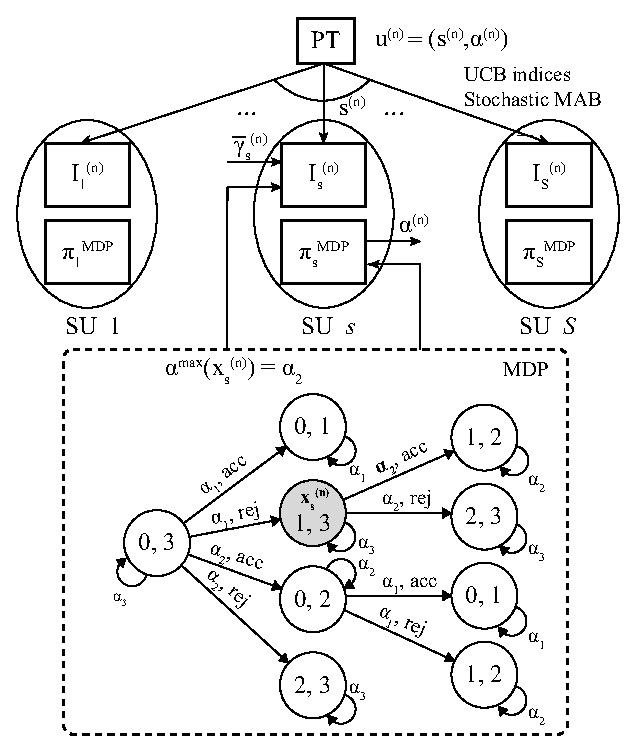
\includegraphics[scale=0.9]{Esquema.eps}
\caption{MAB-MDP algorithm for $S$ SUs and $A=3$ possible offers . Each SU is chosen according to a MAB and the offer according to an MDP. ``acc'' represents the event that the offer is accepted and ``rej'' that it is rejected.}
\label{fig:Esquema}
\vspace{-1.5em}
\end{figure}

\textbf{SU representation in the reduced MAB}. In a classic stochastic MAB, rewards when pulling an arm are drawn from a probability distribution associated to that arm. Proposed policies in the literature compute an index for each arm (dependent on that arm only), $I_s^{(n)}$, and dictate to pull the arm with the highest index on each decision round. A commonly used family of index policies are the Upper Confidence Bound (UCB) policies proposed by \cite{ref:Auer2002}. 
%Let $W^{n}_s$ denote the subsequence of $W^{n}$ corresponding to the rewards obtained from SU $s$.
The index of these policies consists of the sample average reward obtained from arm $s$ up to round $n$, plus an additional term, the \textit{Upper Confidence Bound, (UCB)} related to the uncertainty of that estimation. 

Note that, in our case, $W$ depends not only on $s$ but also on $\alpha$: $W^{(n)}(s,\alpha) = (1-\alpha)\text{log}(\Gamma_s^{(n)})$. When pulling an arm $s$ and offering $\alpha$, the reward is drawn from the Gaussian distribution $\text{log}(\Gamma_s) \sim N(\mu_{\gamma_s},\sigma_{\gamma_s})$, multiplied by a constant $(1-\alpha)$. 
Given the state of SU $s$ at round $n$, $x_s^{(n)}$, we characterize the SU in the reduced MAB by its \textit{best achievable offer} $\alpha^{\text{min}}(x_s^{(n)})$, denoting the minimum $\alpha \in \mathcal{A}_s$ in state $x_s^{(n)}$ with positive belief of being accepted and also being achievable by the offer selection policy $\pi_s^{\text{MDP}}$.\footnote{For a policy $\pi_s^{\text{MDP}}$ that ends up exploring all the offers of an SU, $\alpha^{\text{min}}(x_s^{(n)})$ is simply the lowest $\alpha$ not rejected for the current state $x_i$. For more conservative policies that may dictate not to explore all offers, $\alpha^{\text{min}}(x_s^{(n)})$ is the lowest $\alpha$ that policy is willing to explore given the state $x_s^{(n)}$. The complete notation would be $\alpha^{\text{min}}(x_s^{(n)},\pi_s{\text{MDP}})$ but we use the former to improve readability.} Let us apply this SU characterization in the UCB index for Gaussian distributions shown in \cite{ref:Auer2002}:
\begin{equation}\label{index}
I_{s}^{(n)} = \hat{W}^{(n)}_s + 4 \hat\sigma_{W_{s}}(x_s^{(n)})\sqrt{\frac{\ln(n_{\left\{W>0\right\}} + 2)}{n_s+1}}
\end{equation}
where $\hat{W}^{(n)}_s$ is the best sample average reward of arm $s$ by round $n$, and $\hat\sigma_{W_{s}}(x_s^{(n)})$ is the best standard deviation of the rewards of arm $s$, $n_s$ is the number of times arm $s$ has been pulled up to round $n$, and $n_{\left\{W>0\right\}} $ is the number of rounds in which the PT obtained a positive reward from any SU. Since $s$ is characterized by its best achievable offer in state $x_s^{(n)}$, we have that $\hat{W}_s^{(n)} = (1-\alpha^{\text{min}}(x_s^{(n)}))\overline\gamma_s^{(n)}$ and $\hat\sigma_{W_s}(x_s^{(n)}) = (1-\alpha^{\text{min}}(x_s^{(n)}))\sigma_{\gamma_s}$, with $\overline\gamma_s^{(n)}$ and $\sigma_{\gamma_s}$ denoting the sample mean and known standard deviation of $\gamma_s$, respectively.

Given the UCB index in \cite{ref:Auer2002}, in practice, it can be empirically checked that removing factor $4$ from the upper confidence bound yields a significantly lower regret, while still achieving convergence. 

We proceed to give a detailed \textbf{description of the MAB - MDP algorithm}. Its diagram can be found in Fig. \ref{fig:Esquema}. Initially, for each SU $s \in \mathcal{S}$:
\begin{enumerate}
\item The PT computes the exploration-exploitation policy $\pi_s^{\text{MDP}}$ for the offers $\alpha \in \mathcal{A}_s$. 
\item Given that policy, for the initial state $x_s^{(0)} = (0,A)$, the PT computes the best achievable offer $\alpha^{\text{min}}(x_s^{(0)})$ of each SU. The PT chooses that offer as representative of the SU. 
\item With $\alpha^{\text{min}}(x_s^{(0)})$ and the initial sample of the SNR $\gamma^{(0)}_s$,
%\footnote{We could also leverage this constraint by simply assuming an initial belief (with much uncertainty) about an SU. However, this initial sample is a common practice in most multi-armed bandit algorithms, whose initialization is by pulling all arms first.}
the PT builds the UCB index $I_{s}^{(0)}$ (\ref{index}).
\newcounter{enumTemp}
\setcounter{enumTemp}{\theenumi}
\end{enumerate}
Then, on each round $n$:
\begin{enumerate}
\setcounter{enumi}{\theenumTemp}
\item The PT selects the SU $z$ with the highest UCB index $I_{z}^{(n)}$ and the offer $\alpha_a \in \mathcal{A}_z$ is indicated by the MDP policy $\pi_z^{\text{MDP}}$.
\item If the SU \textit{rejects} the offer, the PT updates its knowledge state (MDP) $x_z^{(n+1)}$ and checks if $\alpha^{\text{min}}(x_z^{(n+1)}) \neq \alpha^{\text{min}}(x_z^{(n)})$. If that is the case, the PT computes $I_{z}^{(n+1)}$ according to (\ref{index}). Otherwise, $I_{z}^{(n+1)} = I_{z}^{(n)}$.
%(the average reward $\overline{W}_s^{(n)}$ and standard deviation $\overline\gamma_s^{(n)}$ get multiplied by the new $(1-\alpha^{\text{min}}(x_{i^{(n)}}))$ factor).
\item If the SU \textit{accepts}, the PT updates $x_z^{(n+1)}$, and sets $n_z =n_z+1$. The indices $I_{s}$ for all $s\in\mathcal{S}$, are also updated because $n_{\left\{W>0\right\}}  = n_{\left\{W>0\right\}}+1$ after the PT receives a positive reward.\footnote{In a classic stochastic MAB, every arm pull increases $n_{\left\{W>0\right\}}$  because every arm pull gives a positive reward from a probability distribution. This is not our case due to the rejection of offers.}
\end{enumerate}

Note that it cannot be assured that this algorithm performs a fully optimal learning. An optimal learning algorithm would imply solving an MDP comprising all the information gathered by the PT. Our MAB-MDP algorithm decomposes the learning problem into two simpler sub-problems (the MAB and the MDP). Each sub-problem can be solved very efficiently because it uses only partial information about the global system. Despite its simplicity, MAB-MDP shows a remarkably low regret in numerical evaluation.
    % \STATE SU $s$ send $\gamma_s^{(0)}$ to the PT
    % \STATE $[{M_s^*},\pi_s^{\text{SPR}}] \leftarrow Frontier Algorithm(\mathcal{X}_s,\mathcal{A}_s,P)$   
    % \STATE $J_s^{(0)} = \gamma_{s}^{(0)}+4\sigma_{\gamma_s}\sqrt{\frac{\ln{(n_{\left\{W>0\right\}}+2)}}{n_s^{(n)}+1}}$    
    % \STATE $M_s^{(0)} \leftarrow M_s^*J_s^{(0)}$
    % \STATE $x_s^{(0)} \leftarrow (0,A)$

\begin{algorithm}
\caption{MAB-MDP algorithm in pseudo-code}
\label{code:TLP}
\begin{algorithmic}
  \FORALL{$s \in \mathcal{S}$}
    \STATE SU $s$ send $\gamma_s^{(0)}$ to PT
    \STATE $\pi_s^{\text{MDP}} \leftarrow Policy Iteration(\mathcal{X}_s,\mathcal{A}_s,P_s)$
    \STATE $x_s^{(0)} \leftarrow (0,A)$
    \STATE $\overline{W}_s^{(0)}\leftarrow (1-\alpha^{\text{min}}(x_s^{(0)}))\gamma_s^{(0)}$ 
    \STATE $\hat\sigma_{W_s}(x_s^{(0)}) \leftarrow (1-\alpha^{\text{min}}(x_s^{(0)}))\sigma_{\gamma_s}$
    \STATE $n_{\left\{W>0\right\}}, n_s^{(n)}, n \leftarrow 0$
    \STATE $I_{s}^{(0)} = \overline{W}^{(0)}_s + 4 \sigma_{W_{s}}(x_s^{(0)})\sqrt{\frac{\ln(n_{\left\{W>0\right\}} + 2)}{n_s+1}}$
  \ENDFOR
  \LOOP
    \STATE $z \leftarrow \underset{s}\max\text{ }I_s^{(n)}$
    \STATE $\alpha_a \leftarrow \pi_z^{\text{MDP}}(x_z^{(n)})$
    \STATE PT offers $\alpha_a$ to SU $z$
    \IF[SU rejects] {$\alpha_a < \alpha_{z}^{th}$} 
      \STATE collect reward  $0$
      \STATE $x_z^{(n+1)} \leftarrow (a,x_z^{(n)}(2))$ 
      \STATE $\overline{W}_z^{(n+1)}\leftarrow (1-\alpha^{\text{min}}(x_z^{(n+1)}))\overline{\gamma}_z^{(n)}$
      \STATE $\hat\sigma_{W_z}(x_z^{(n+1)}) \leftarrow (1-\alpha^{\text{min}}(x_z^{(n+1)}))\sigma_{\gamma_z}$
      \STATE $I_{z}^{(n+1)} \leftarrow \overline{W}_z^{(n+1)} + 4\sigma_{W_z}(x_z^{(n+1)}) \sqrt{\frac{\ln(n_{\left\{W>0\right\}} + 2)}{n_z+1}}$ 
      \FORALL{$s \in \mathcal{S}, s \neq z$}
        \STATE $I_{s}^{(n+1)} \leftarrow I_{s}^{(n)}$
        \STATE $x_s^{(n+1)} \leftarrow x_s^{(n)}$
      \ENDFOR
    \ELSE
      \STATE collect reward $(1-\alpha_a)\log(\Gamma_z^{(n)})$
      \STATE $x_z^{(n+1)} \leftarrow (x_z^{(n)}(1),a)$
      \STATE $\overline{\gamma}_{z}^{(n+1)} \leftarrow \frac{\overline{\gamma}_{z}^{(n)}n_z+\gamma_z^{(n)}}{n_z+1}$  
      \STATE $\overline{W}_z^{(n+1)}\leftarrow (1-\alpha^{\text{min}}(x_z^{(n)}))\overline{\gamma}_z^{(n+1)}$
      \STATE $n_z \leftarrow n_z + 1$
      \STATE $n_{\left\{W>0\right\}} \leftarrow n_{\left\{W>0\right\}} + 1$
      \FORALL{$s \in \mathcal{S}$}
        \IF{$s \neq z$} 
          \STATE $x_s^{(n+1)} \leftarrow x_s^{(n)}$
          \STATE $\overline{W}_s^{(n+1)}\leftarrow \overline{W}_s^{(n)}$
        \ENDIF
        \STATE $I_{s}^{(n+1)} \leftarrow \overline{W}_{s}^{(n+1)} + \hat\sigma_{W_s}(x_s^{(n)}) \sqrt{\frac{\ln(n_{\left\{W>0\right\}} + 2)}{n_s+1}}$
      \ENDFOR
    \ENDIF
    \STATE $n \leftarrow n + 1$
  \ENDLOOP
\end{algorithmic}
\end{algorithm}
%This formulation does not perform an optimal learning of both the average SNR $\mu_{\gamma_s}$ and the type of an SU. The MDP of each arm does not consider the possibility of the PT of choosing a different SU, or how interacting several times with the same has an impact on the estimate $\overline{\gamma_s}^{(n)}$, although this is captured in some way by the stochastic MAB. And viceversa in the MAB decision: when choosing the SU, the UCB index is not considering all the information the PT knows about the SUs acceptance of offers, just the maximum offer $(1-\alpha_{x_i}^{min})$ the PT believes it can get from each SU. But the exploration-exploration trade-off in discovering the optimal offer is considered by the MDP.

\section{Super-UCB}\label{sec:Super}
The MAB-MDP algorithm of previous section is based on an stochastic MAB. In this section we follow the markovian MAB approach. Our objective is to profit from all the information gathered about the SU types, instead of considering only their best achievable offer.

For the classic markovian MAB with independent arms in which the decision-maker (DM, the PT in our scenario) selects an arm to play and receives a random reward from a Markov chain, Gittins \cite{ref:Gittins2011} developed an index policy proven to be optimal if the transition probabilities are known.
The computation of the indices for each state of each arm is performed offline. 
The online sequential decision is as simple as in the stochastic MAB index policies: on each decision stage, the DM has to pull the arm with the highest index for their current states. 
Then, the state of the pulled arm changes and so does the index of that arm, which is replaced by the one associated to the new state. 

\textbf{Superprocess}. 
As we are grouping the arms of the MAB by SU, the rewards when choosing an SU are not drawn from Markov reward chains but from Markov Decision Processes (MDP). The PT does not only select which SU to interact with (pulling an arm) but also which offer to make (selecting an action of the MDP). 
If we consider the SUs as independent, this problem can be formulated as an extension to MABs called \textit{superprocess}. P. Whittle \cite{ref:Whittle1980} extended the Gittins index policies to superprocesses. Regarding the selection of action for the MDP, there are different choices that we discuss later.


%Note that the MDPs of the arms in this case will differ from the MDP described in eq. (\ref{eq:MDP}) in that now we are not focusing only in the policy for the offers. This MDP now
Ideally, such MDP of an arm should encode all information or beliefs the PT has about a SU, that is, both the acceptance and rejection of offers, and the samples of $\gamma_s^{(n)}$. 
Unfortunately, including the information about $\gamma_s^{(n)}$ would lead to a continuous-state MDP which is intractable in practice. 
Combining the superprocess with Approximate Dynamic Programming techniques is not an option either: as it is shown in \cite{ref:Pandey2007}, the approximations obtained for Gittins indices are not tight enough (not even to be used as heuristics). How could we integrate the uncertainty about $\mu_{\gamma_s}$ in the superprocess, without making the state space explode?. We propose an approximate method by including the PT's beliefs about $\mu_{\gamma_s}$ in the reward of the MDP in the form of an UCB index, instead of including them as state variables. Then, in every round in which the UCB indices get updated, that is, rounds in which the PT's beliefs about $\mu_{\gamma_s}$ change, the PT recomputes the superprocess using the new UCB indices in the rewards of the MDPs, obtaining a new set of Gittins indices for all states.


\textbf{Solution to the superprocess.} In order to obtain the Gittins index for state $x_i$ of an arm $s$, Whittle introduces a retirement action into the Bellman equation.
The retirement action leads to a ficticious final state with a unique reward $M$. Then, the value of state $x_i$ in round $n$, $V_s(x_i,M)$, is obtained by solving:
\begin{equation}\label{eq:MDPret}
\begin{split}
&V_s(x_i,M) = \max\left\{M, \vphantom{ \sum_{x_{j}}}\right.\\
&\left.\max_{\alpha_a \in \mathcal{A}_s} \sum_{x_{j} \in \mathcal{X}_s} P_s(x_i,x_{j},\alpha_a)\left(h_s^{(n)}(x_{j},\alpha_a)+\delta V_s(x_{j},M)\right)\right\}
\end{split}
\end{equation}
where $h_s^{(n)}$ denotes the reward function at round $n$, associated to a transition of the MDP of SU $s$, and it is defined as follows:
\begin{equation}
h_s^{(n)}(x_{j},\alpha_a) = 
\begin{cases}
    (1 - \alpha_a) J_s^{(n)} & \text{for } a = x_j(2)\\
    0 & \text{for } a = x_j(1)
   \end{cases}
\end{equation}

and $J_s^{(n)}$ denotes an UCB index of the form $J_s^{(n)} = \left(\overline{\gamma}_{s}^{(n)}+4\sigma_{\gamma_s}\sqrt{\frac{\ln{(n_{\left\{W>0\right\}}+2)}}{n_s+1}}\right)$.
The \textit{Gittins index} $M_s^{(n)}(x_i)$ for SU $s$ in state $x_i$ and round $n$ is the smallest $M$ that makes the DM indifferent between taking the retirement action or continuing in the sequential decision problem. 
The retirement action and state could be thought of as the reward obtained by switching to a generic project: it symbolizes the reward that could be achieved by the other arms.

So as to find the Gittins indices $M_s^{(n)}(x_i), \forall x_i \in \mathcal{X}_s$, (\ref{eq:MDPret}) has to be repeatedly solved for different values of $M$. Following the approach in \cite{ref:Brown2013}, we can formulate (\ref{eq:MDPret}) as a linear program \cite{ref:Bertsekas2005} and use the techniques of parametric linear programming with parameter $M$.
Let $\boldsymbol{v}_s$ denote the vector of values $V_s(x_i,M), x_i \in \mathcal{X}_s$. The corresponding linear program to (\ref{eq:MDPret}) for SU $s$ in round $n$ is: 
\begin{equation}
\begin{split}
  &\underset{v_s}{\text{minimize }}\sum_{x_i \in \mathcal{X}_s} v_s(x_i)\\
  &\text{subject to }v_s(x_i) \geq \sum_{x_j \in \mathcal{X}_s}  P_s(x_i,x_j,\alpha_a)(h_s^\text{(n)}(x_i,x_j,\alpha_a)\\
  &\hphantom{\text{subject to }v_s(x_i) \geq \sum_{x_j \in \mathcal{X}_s} P_s}+\delta v_s(x_j)), \forall x_i \in \mathcal{X}_s,\alpha_a \in \mathcal{A}_s\\
  &\hphantom{\text{subject to }}v_s(x_i)\geq M \text{,    }\forall x_i \in \mathcal{X}_s
\end{split}
\end{equation}

$V_s(x_i,M)$ is known to be piecewise linear, increasing, and convex in $M$ \cite{ref:Brown2013}. Obtaining the value of $V_s(x_i,M)$, then, consists of finding the slopes and breaking points of the pieces. Using the Gaas-Saaty algorithm for parametric linear programming \cite{ref:Gass1955}, the authors of \cite{ref:Brown2013} proposed the \textit{Frontier Algorithm} to compute the Gittins indices $M_s^{(n)}(x_i)$. The Gaas-Saaty algorithm is a variation of the traditional simplex method for linear programs.

Given (\ref{eq:MDPret}) and the particular form of $h^{(n)}$, there is no need to recompute the superprocess on each round because of the changes in $J_s^{(n)}$. It is easy to see that $J_s^{(n)}$ is a common factor in every term of the sum of (\ref{eq:MDPret}) and thus, it is enough to solve the equation once per SU for a generic $J_s^{(n)} = 1$. If we denote that generic Gittins index by $M_s^*(x_i)$, then we can obtain the Gittins index in round $n$ by $M_s^{(n)}(x_i) = M_s^*(x_i)J_s^{(n)}$. This fact greatly reduces the computation overhead of the algorithm, as the superprocess only has to be solved offline once.

\textbf{Offer selection policy.} Regarding the action to take on a given state for an arm, there are different choices.
Whittle - Gittins index policy for superprocesses turns out to be optimal only if there is a dominant action $\alpha_s^{\text{DOM}}(x_i)$ for each arm and state that achieves the maximum in (\ref{eq:MDPret}) for all values of $M \in [0,M_s^*(x_i)]$. 
If that is the case, the action indicated by the policy is the dominant action. In our case, however, the action indicated by the policy solving (\ref{eq:MDP}), changes with the retirement value. 
This means that the choice of action for a given SU depends on what the PT knows about the others (\textit{i.e} depending on the types of the other SUs, the PT may decide to explore more or less a particular SU). Thus, it is suboptimal to consider each SU in isolation when deciding on the offer to make.
Nevertheless, even for this suboptimal case, the Gittins - Whittle's policy can still be used as an heuristic, providing tight upper bounds (< 2\%) on the values of $V_s(x_i)$ (eq. (\ref{eq:MDPret})) as reported by \cite{ref:Brown2013}.
For the suboptimal cases, \cite{ref:Pandey2007} suggests to choose the actions that maximize $V_s(x_i, M_s^*(x_i))$. 
However, as noticed by \cite{ref:Brown2013} as well as in our simulations, such policy leads to under-exploration of a SU. To solve this issue, it suffices to set to zero the retirement reward. Therefore, the offer selection policy is determined by the actions maximizing $V_s(x_i,0)$ in the MDP in (\ref{eq:MDP}). We will denote such policy by $\pi_s^{\text{SPR}}$. The Frontier Algorithm provides all the previously mentioned policies. 

\textbf{Description of the Super-UCB algorithm.}
\begin{figure}[!t]
\centering
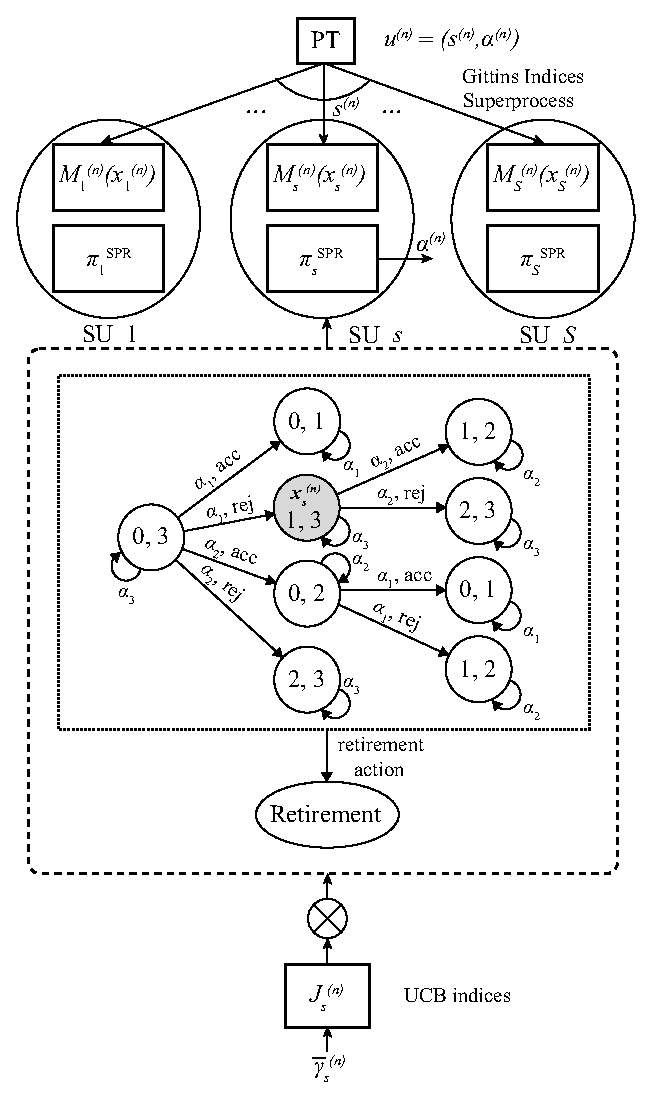
\includegraphics[scale=0.8]{esquemaSuper.eps}
\caption{Super-UCB algorithm for $S$ SUs and $A=3$ possible offers. SUs and offers are chosen according to a MAB superprocess, whose reward includes an UCB index as a factor. ``acc'' represents the event that the offer is accepted and ``rej'' that it is rejected.}
\label{fig:esquemaSuper}
\end{figure}
Its diagram can be found in Fig. \ref{fig:esquemaSuper}. Initially, for each SU $s \in \mathcal{S}$:
\begin{enumerate}
\item We obtain the generic Gittins indices $M_s^*(x_i)$ and the offer selection policy $\pi_{s}^{SPR}$ for every state $x_i$ of SU $s$, solving (\ref{eq:MDPret}) with the Frontier Algorithm.
\item The PT computes the UCB index $J_s^{(0)}$ with the initial samples $\gamma_s^{(0)}$, and also computes the Gittins indices $M_s^{(0)}$.
\newcounter{enumTempB}
\setcounter{enumTempB}{\theenumi}
\end{enumerate}
Then, on each round $n$:
\begin{enumerate}
\setcounter{enumi}{\theenumTempB}
\item The PT selects the SU $z$ with the highest Gittins index $M_z^{(n)}(x_z^{(n)})$, $z \in \mathcal{S}$, and the offer $\alpha_a \in \mathcal{A}_s$ indicated by $\pi_{z}^\text{SPR}$.
\item If the SU \textit{rejects} the offer, the PT updates its current knowledge state $x_{z}^{(n+1)}$, and the SU is represented by the Gittins index $M_z^{(n+1)}(x_z^{(n)})$ of the new state.
%(the average reward $\overline{W}_s^{(n)}$ and standard deviation $\overline\gamma_s^{(n)}$ get multiplied by the new $(1-\alpha^{\text{min}}(x_{i^{(n)}}))$ factor).
\item If the SU \textit{accepts}, the PT updates $x_{z}^{(n+1)}$, the SU is represented by the Gittins index $M_z^{(n+1)}(x_z^{(n)})$ of the new state, and the PT sets $n_{z}=n_{z}+1$. The indices $J_{s}$ for all $s\in\mathcal{S}$, are also updated because $n_{\left\{W>0\right\}}  = n_{\left\{W>0\right\}}+1$ after the PT receives a positive reward.
\end{enumerate}

Note that it is still not assured that the algorithm performs fully optimal learning, which, as we have already seen, is intractable.
Nevertheless, \textit{Super-UCB makes a more effective use of the available information with respect to the MAB-MDP algorithm.} This is reflected in a regret gap as shown in Section \ref{sec:Num}. 
When choosing which SU $s$ to bargain with, Super-UCB takes into account all the PT knowledge about the type of a SU, while MAB-MDP represents each SU by its best achievable offer (or best possible type given the observations). 
Let us imagine two SUs, one which the PT knows it accepts at least type-2 offers but does not know about type-1, and another which is completely unknown. 
In MAB-MDP, both will be represented by the best achievable offer in that state, the type-1 offer. Choosing one SU or the other will be determined by the one that shows the higher UCB index (related to the samples of $\gamma_s$).
MAB-MDP algorithm, thus, tends toward an over-exploration of different SUs.
If we try to include all the information about SU types in the UCB indices of MAB-MDP, representing each SU by averaging over its possible types, it results in a PT more reluctant to try an unknown SU, since its average will be lower than a better known SU (that may not be the optimal). That policy tends toward more exploitation of each particular SU and the results in terms of regret are notably worse. \textit{Super-UCB, however, can use the information about SU types in a more balanced way thanks to the retirement action in the superprocess formulation}: when computing the offer selection policy, the superprocess takes into account the possibility of stop exploring a SU and switching to another that may return higher rewards, and that affects the value of the states of SUs. On the contrary, an MDP offer selection policy is equivalent to considering zero retirement value and hence the reluctance to explore unknown SUs.  

\begin{algorithm}
\caption{Super-UCB algorithm in pseudo-code}
\label{code:FA_UCB}
\begin{algorithmic}
  \FORALL{$s \in \mathcal{S}$}
    \STATE SU $s$ send $\gamma_s^{(0)}$ to the PT
    \STATE $[{M_s^*},\pi_s^{\text{SPR}}] \leftarrow Frontier Algorithm(\mathcal{X}_s,\mathcal{A}_s,P_s)$   
    \STATE $n_{\left\{W>0\right\}}, n_s^{(n)}, n \leftarrow 0$
    \STATE $J_s^{(0)} = \gamma_{s}^{(0)}+4\sigma_{\gamma_s}\sqrt{\frac{\ln{(n_{\left\{W>0\right\}}+2)}}{n_s^{(n)}+1}}$    
    \STATE $M_s^{(0)} \leftarrow M_s^*J_s^{(0)}$
    \STATE $x_s^{(0)} \leftarrow (0,A)$
  \ENDFOR
  \LOOP
    \STATE $z \leftarrow \underset{s}\max{\text{ }}M_s^{(n)}(x_s^{(n)})$
    \STATE $\alpha_a$ $\leftarrow \pi_s^{SPR}(x_z^{(n)})$
    \STATE PT offers $\alpha_a$ to SU $z$
    \IF[SU rejects] {$\alpha_a < \alpha_{z}^{th}$} 
      \STATE collect reward  $0$
      \STATE $x_z^{(n+1)} \leftarrow (a,x_z^{(n)}(2))$
      \STATE $x_s^{(n+1)} \leftarrow x_s^{(n)} \text{ }\forall s \neq z$
    \ELSE
      \STATE collect reward $(1-\alpha_a)\log(1+\Gamma_{z}^{(n)})$
      \STATE $x_{z}^{(n+1)} \leftarrow (x_z^{(n)}(1),a)$ 
      \STATE $\overline{\gamma}_{z}^{(n+1)} \leftarrow \frac{\overline{\gamma}_{z}^{(n)}n_z+\gamma_z^{(n)}}{n_z+1}$  
      \STATE $n_{z} \leftarrow n_{z} + 1$
      \STATE $n_{\left\{W>0\right\}} \leftarrow n_{\left\{W>0\right\}} + 1$
      \FORALL{$s \in \mathcal{S}$}
        \IF{$s \neq z$} 
          \STATE $\overline{\gamma}_{s}^{(n+1)} \leftarrow \overline{\gamma}_{s}^{(n)}$  
          \STATE $x_s^{(n+1)} \leftarrow x_s^{(n)}$
        \ENDIF   
        \STATE $J_s^{(n+1)} \leftarrow \overline{\gamma}_{s}^{(n+1)} + 4\sigma_{\gamma_s} \sqrt{\frac{\ln{(n_{\left\{W>0\right\}}+2)}}{n_s+1}}$
        \STATE $M_s^{(n+1)} \leftarrow M_s^*J_s^{(n+1)}$
      \ENDFOR
    \ENDIF
    \STATE $n \leftarrow n+1$
  \ENDLOOP
\end{algorithmic}
\end{algorithm}

% \section{Stochastic bandit setting}\label{sec:Sto}
% In this scenario, we assume that the PT does not have a full knowledge a priori of the channel gain between the SU and the PR. 
% Even if we assume that every SU would be able to have a perfect estimation of the SNR at the PU receiver prior to any transmission, it is unlikely that this information would be shared with the PT, as we argued in the introduction.
% Not assuming ``how good a SU is'' in terms of reward also allows for the characterization of some strategic behavior from the SUs, by modeling them more complex belief distributions. 
% However, we will consider myopic SUs and the variation on the SNR is due to block shadowing in the channel.
% The PT will not only have to learn about the offers a particular SU accepts, but also the statistics of the channel, so as to choose the combination of channel quality and SU type that maximizes the PT's utility function. 
% Here, we have to distinguish two types of learning, using the naming convention of \cite{ref:Powell2012}: 
% \begin{itemize}
% \item Experiential learning. The PT updates its beliefs based on the samples it observes of the random variables (the rewards, the received SNR at the PR).
% \item Anticipatory learning. Learning is taken into account in the policy. The PT's decision will be influenced by the knowledge gain it will have when observing a random variable.
% \end{itemize}

% \textbf{Sequential superprocess.}
% An initial approach we considered to address this scenario was to solve a superprocess in a sequential way, on each decision round, including experiential learning by using statistical inference.
% It works as follows:
% \begin{enumerate}
% \item We assume that the PT knows the distribution that models the received SNR from every SU (the PT could extract such knowledge from previous history) but it does not know their parameters. In our simulations, we will further assume that these distributions are the same for every SU, with same known variance (taken, for example, from empirical measurements) but unknown mean. In this case, 
% \begin{equation}
% \gamma_s(dB) \sim \mathcal{N}(\mu_s,\sigma)
% \end{equation}
% \item We could also assume that the PT has an initial belief about the value of the unknown means, expressed as a probability distribution over values (\textit{prior distribution}). In our case, it should be conveniently expressed as a normal distribution:
% \begin{equation}
% \mu_s \sim \mathcal{N}(\mu_s^0,\sigma_s^0)
% \end{equation}
% Initially, the PT receives a sample of the received SNR of every SU in the system. In our case, we use it to create the prior distribution. We will consider our initial belief to be centered around the sample and our uncertainty be the variance of the sample.
% \item The PT will consider the mean of the prior distribution as the ground truth for the mean SNR value of each SU, and will use it in the reward for the superprocess as formulated in the previous section. After computing the Gittins indexes and obtaining the policies, the PT will choose the SU and offer indicated by the Frontier Algorithm. 
% \item If the offer is accepted, the PT updates the state of the SU accordingly (now the PT knows that offer is accepted) and observes the reward. It uses the observed SNR to update the prior distribution of belief, obtaining a new probability distribution known as the \textit{posterior distribution}. By choosing convenient probability distributions (assuming a normal distribution for the samples, expressing the beliefs with a normal distribution), the update equations are simple and the posterior distribution is the same distribution than the prior. Then,
% \begin{equation}
% \mu_s \sim \mathcal{N}(\mu_s^1(\mu_s^0,\gamma_s^1),\sigma_s^1(\sigma_s^0))
% \end{equation}
% \item For the next decision stage, the PT again uses the mean of the belief distribution as the ground truth, (updated for the SU of the previous round), re-computes the Gittins indexes of the states of that SU and chooses SU and action as usual.
% \item If the offer is rejected, the state of the arm corresponding to that SU changes. There is no change in the SNR beliefs however (as the PT receives no sample of SNR).In the next decision round, the PT again chooses the SU with highest index (which may be the same SU with a different offer or a different SU). 
% \end{enumerate}

% Both experiential and anticipatory learning processes take place when learning the type of the SU. 
% The arms MDPs, which model that learning, take into account the value of information (how the beliefs about the type of the SU are going to change as a consequence of every action, anticipatory learning) and after the observation of the acceptation or rejection from the SU, the knowledge states evolve accordingly (experiential learning). 
% Nevertheless, the PT is not doing any anticipatory learning about the probability distribution of the SNRs. 
% It will simply accept the mean of the belief distribution about every SU as the true average reward of it, no matter how inaccurate it is.
% This could end up in the PT choosing a suboptimal arm (s,$\alpha$) with high probability.
% For example, if the first sample from ``the best SU in average'' is bad, the index policy may never dictate to bargain with it: its associated Gittins indexes may be low compared to those of the other SUs. 
% As a consequence, the PT may underestimate the optimal SU and never choose it. 

% However, it is more difficult for the PT to choose a suboptimal arm because of an initial overestimation of the SNR. 
% After interacting with the overestimated SU, it will eventually learn the true average received SNR. 

\section{Numerical results}\label{sec:Num}
In addition to the MAB-MDP, we use two more algorithms as benchmarks for Super-UCB: an $\epsilon$-greedy algorithm and a standard superprocess which we call Super-0CB. We evaluate them over time, versus the standard deviation on $\sigma_{\gamma_s}$, number of SUs and number of offers. We also observe the robustness of MAB-MDP and Super-UCB against misestimations of $\sigma_{\gamma_s}$.
\textbf{Comparison with $\epsilon$-greedy}.
Given the main features of our proposed mechanism (real-time operation and exploration-exploitation tradeoff), the best candidates for comparison are the families of reinforcement learning heuristics \cite{ref:Vermorel2005} known as $\epsilon$-greedy policies.
Specifically, we will compare our algorithm to the $\epsilon$-descending strategy. 
This strategy chooses the alternative $u = (s,\alpha)$ with best expected reward with probability $1-\epsilon^{(n)}$, and performs random exploration with probability $\epsilon^{(n)}$, which, in each round $n$, takes the value $\epsilon^{(n)} = \epsilon^{(0)}/n$, or $\epsilon^{(n)} = \epsilon^{(0)}\ln(n)/n$ for a log-descending variant, where $\epsilon^{(0)}$ is a tunable parameter. The alternative $u$ is chosen according to: $u = (s,\alpha) = \argmax_{s,\alpha} (1-\alpha)\overline{W}^{(n)}_s P(\alpha_s^{\text{th}} \leq \alpha)$.
As it is noted in the literature \cite{ref:Auer2002,ref:Vermorel2005}, the $\epsilon$-descending greedy strategy performs as well as (and most of the time, even better than) many other complex policies. 
Its main drawback is that the $\epsilon^{(0)}$ parameter has to be carefully chosen and there is little that can be said theoretically about its optimal value except for distributions with support on $[0,1]$ (see \cite{ref:Auer2002}). 
Based on empirical tests of a wide range of values for $\epsilon^{(0)}$, we set it to $10$ for all figures. 

\textbf{Comparison with a superprocess without upper confidence bounds (Super-0CB)}.
We also compare to a sequential computation of the superprocess in (\ref{eq:MDPret}) with $J_s^{(n)} = \overline{\gamma}_s^{(n)}$ which we will call \textit{Super-0CB}. This is equivalent to compute the Gittins indices on every round $n$ assuming that the true values of $\mu_{\gamma_s}$ for upcoming rounds are the sample means observed up to round $n$, that is, zero confidence bound. 
We set the discount factor $\delta$ of MAB-MDP, Super-UCB, and Super-0CB to 0.98.
We summarize the information taken into account by each algorithm in Table \ref{Table:info}.
\begin{table}
\begin{threeparttable}
\caption{Summary of the information exploited by each algorithm}
\label{Table:info}
\begin{tabulary}{8.5cm}{|l|C|C|C|C|}
\hline
& $\overline\gamma_s$ & $\sigma_{\gamma_s}$ & Possible SU types for SU selection & Possible SU types for offer selection \\ \hline
$\epsilon$-greedy & \checkmark & $\times$ & / & / \\ \hline
Super-0CB         & \checkmark & $\times$ & \checkmark & \checkmark \\ \hline
MAB-MDP           & \checkmark & \checkmark & / & \checkmark \\ \hline
Super-UCB         & \checkmark & \checkmark & \checkmark & \checkmark \\ \hline
\end{tabulary}
\begin{tablenotes}
\item \hspace{2em} \checkmark = exploited, / = partly exploited, $\times$ = not exploited
\end{tablenotes}
\end{threeparttable}
\end{table}

\subsubsection{Performance over time}
\begin{figure}[!t]
\centering
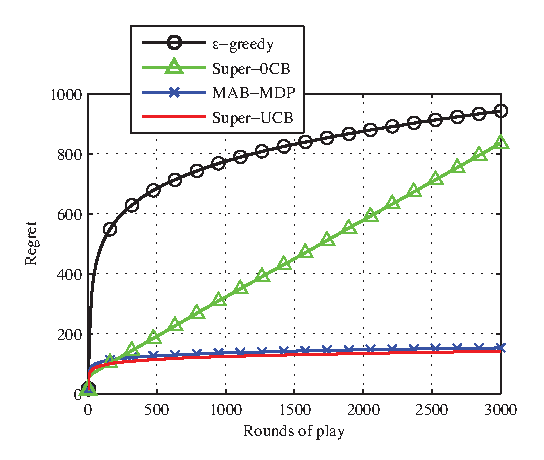
\includegraphics{stoVsT.eps}
\caption{Regret over time for the MAB-MDP, Super-UCB, Super-0CB and the $\epsilon$-greedy algorithms. The results are averaged over 2000 independent experiments.}
\label{fig:stoVsT}
\end{figure}

Fig. \ref{fig:stoVsT} shows the performance of our two proposals MAB-MDP and Super-UCB over time compared to the $\epsilon$-greedy, for $S=7$ SUs and $A=7$ possible $\alpha$ offers.
The standard deviation of the SNR of each arm $s$ is $\sigma_{\gamma_s} = 5$ dB.

As expected, MAB-MDP and Super-UCB outperform $\epsilon$-greedy because they make a more effective use of information in their decision processes. As it was previously anticipated, the shape of both curves of the MAB-MDP and Super-UCB is the same but with a gap. The reason of this gap is the loss of information in the MAB-MDP algorithm.
% Figure \ref{fig:stoVsT} shows a comparison of our two proposals in the stochastic bandit scenario: the two-layer policy that addresses both anticipatory and experiential learning and the sequential superprocess with upper confidence bounds as rewards. 
% They are compared to the extension of the superprocess policy to experiential learning of SNRs, that is, re-computing the superprocess on each decision stage; and the $\epsilon$-greedy.  
% We consider that the algorithms know the standard deviation of the SNR of each arm, which is 5 dB \footnote{\cite{ref:Goldsmith2009} indicates typical values between 4-13 dB in empirical measurements.}. 

No surprise is also what happens with Super-0CB over time: the regret increases linearly on average due to the cases where the best arm showed bad initial samples and thus, a suboptimal arm is selected. 
It does perform better than the other algorithms in the initial frames simply because it does more exploitation than MAB-MDP and Super-UCB, and still balances exploration and exploitation of the offers of SUs unlike the $\epsilon$-greedy.

\subsubsection{Performance versus standard deviation}

Figure \ref{fig:VsKnownVar} shows the performance of the algorithms versus different values of $\sigma_{\gamma_s}$. The standard deviation for log-normal shadowing vary from 4 to 13 dB depending on the environment, and it is related to the variations of the blockage that objects cause in the signal path \cite{ref:Goldsmith2005}. The higher the deviations, the harder the problem, as the samples of each distribution may not preserve the rank of their mean values, that is to say, bad arms may appear as the best ones and viceversa. The MAB-MDP and Super-UCB standard deviation terms are adjusted accordingly. 

$\epsilon$-greedy and Super-0CB algorithms experience notable performance degradation under high variance. This is because they rely on estimates of the mean reward. As the variance increases, more rounds are needed for the sample mean to converge to the true mean. Nevertheless, due to its random exploration nature, $\epsilon$-greedy manages to eventually find the optimal arm, which is something that cannot be said about Super-0CB and hence its poor results. 
The proposed UCB-based algorithms show certain robustness under high variances, since they take the standard deviation into account when making their decisions. 
 
\begin{figure}[!t]
\centering
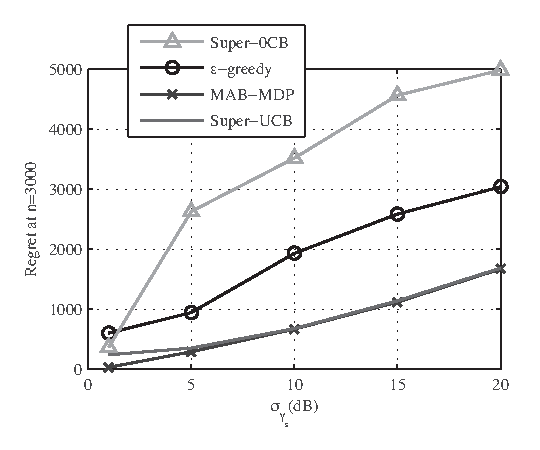
\includegraphics{VsKnownVar.eps}
\caption{Regret at $n = 3000$ for the MAB-MDP and the $\epsilon$-greedy algorithms for different values of the $\sigma_{\gamma_s}$. Mean SNRs and SU types are fixed over experiments. $\boldsymbol{\mu_{\gamma}}=\{35,32.5,32.5,30,30,27,27\}$ and SU types $= \{1,1,1,2,2,3,3\}$.}
\label{fig:VsKnownVar}
\end{figure}

\subsubsection{Performance under mis-estimation of standard deviation}

Fig. \ref{fig:unknownVar} shows the effect of mistestimating the standard deviation $\sigma_{\gamma_s}$ in our algorithms. $\epsilon$-greedy and Super-0CB perform a frequentist inference and therefore does not make use of the variance.

Underestimating or overestimating $\sigma_{\gamma_s}$ in the UCB index implies being less or more optimistic, respectively, about the values of the true average rewards of the SUs, based on the sample means observed. 
Thus, an overestimation implies more exploration of each SU and an increased probability of finding the optimal arm.
An underestimation implies more exploitation of SUs and less exploration. 
As shown in the figure, overestimation is safer than underestimation in terms of regret.
Overestimation causes a slower convergence towards the optimal arm but underestimation could make the algorithm converge to a suboptimal solution, which is associated to linear regret with the number of rounds. The difference between the rewards of the optimal and that suboptimal arm on each round accumulates over time.  
Note that, under severe underestimation, both MAB-MDP and Super-UCB can even do worse than the $\epsilon$-greedy algorithm, but no worse than Super-0CB
Underestimation may be justified in a scenario where the SUs are expected to stay a short time in the coverage area of the PT. 
Then, the PT may be better off sacrificing the search of an optimal arm for exploiting suboptimal arms with ``good enough'' rewards.
%It will have an impact in case of selecting a different prior belief (Bayesian inference): the variances of the initial beliefs about the true means and the assumed variances of the rewards act as ``weights'' when computing the mean. Underestimating the variance of the rewards will give less value than optimal to the empirical samples compared to the initial belief, and overestimating it will cause the opposite effect. The overall effect on the Bayesian inference would also depend on how accurate is the initial belief. 


\begin{figure}[!t]
\centering
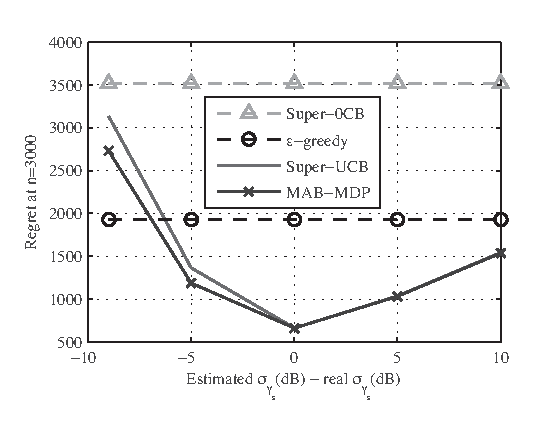
\includegraphics{unknownVar.eps}
\caption{Regret at $n = 3000$ for different estimations of $\sigma_{\gamma_s}$, with the real value of $\sigma_{\gamma_s}$ = 10 dB. Mean SNRs and SU types are fixed over experiments.}
\label{fig:unknownVar}
\end{figure}

\subsubsection{Performance against number of SUs and discretization levels of the offers}

Fig.\ref{fig:VsN} and fig. \ref{fig:VsA} illustrate how regret grows with respect to the optimal policy for the different algorithms when increasing the number of SUs in the system or the granularity of the offers the PT can make.
Note that a higher regret represents worse performance with respect to the optimal policy.
With a higher number of SUs or higher number of possible offers, the ideal reference policy obtains better rewards. 
In short: finding the optimal arm is harder but that optimal arm provides a higher reward than the optimal arm of a scenario with fewer SUs or fewer possible offers. 
That said, both figures show that the proposed algorithms scale well when increasing the size of the problem, as the regret grows dramatically less than for the $\epsilon$-greedy or the basic Super-0CB  
This is because of the more effective use of the available information made by the UCB-based algorithms. 
Moreover, the computational cost or memory requirements do not experience a significant growth, even for the worst case, which is increasing the number of offers. 
The state space of the MDP of an SU, $\mathcal{X}_s$, grows with the number of offers, $A$, as $|\mathcal{X}_s| = A(A+1)/2$, which for a fine-grained range of 20 possible offers becomes 210 states and 20 actions on each state. 
\begin{figure}[!t]
\centering
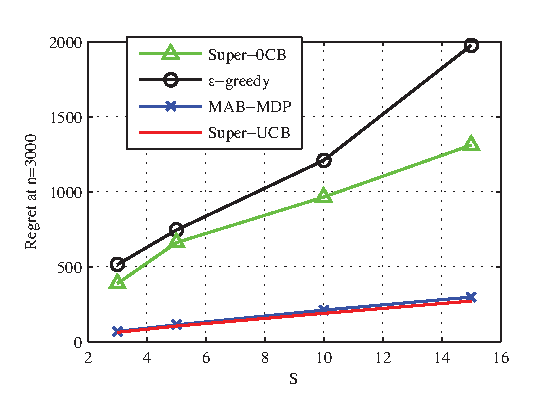
\includegraphics{VsN.eps}
\caption{Regret at $n = 3000$ for different number of SUs, $S$. Number of possible offers $A = 7$.}
\label{fig:VsN}
\end{figure}

\begin{figure}[!t]
\centering
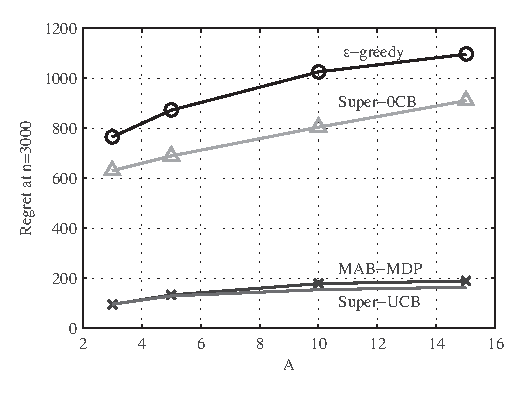
\includegraphics{VsA.eps}
\caption{Regret at $n = 3000$ for different number of possible offers, $A$. Number of SUs $S = 7$.}
\label{fig:VsA}
\end{figure}

\section{Conclusion and future work}\label{sec:Con}
%Brief summary
We have proposed a spectrum trading mechanism in Cooperative Spectrum Sharing using multi-armed bandits, from the perspective of a primary transmitter (PT),  modeling channels under shadowing effects. 
We have focused on a scenario where the PT has no knowledge of the performance of the SUs acting as relays, or about the offers they are willing to accept. 
Our two algorithms, MAB-MDP and Super-UCB have shown to learn payoff-maximizing actions for the PT with little communication or computation overhead. 
%Results
Our numerical results indicate that, despite their simplicity, they significantly outperform the classical exploration-exploitation $\epsilon$-greedy algorithm, with Super-UCB featuring a better overall performance.
They are shown to be robust to inaccuracies in the little information they need and to scale well when the size of the problem increases, \textit{i.e.,} for more SUs and available offers.
%Next
This work can be the starting point to develop more complex scenarios.  
Considering the explosion of MAB variants in the recent literature, as the next steps it would be possible and interesting to study: 1) how to exploit the spatial fading correlation across different SUs, 2) extension of the algorithms to a multiple PT and / or multiple PR case, 3) inclusion of more dimensions to learning, such as learning the staying time of SUs in the PT coverage area or the distribution of the SU types, and 4) inclusion of SU / PU strategic behavior. 